\documentclass{article}
\usepackage[utf8]{inputenc}
\usepackage{hyperref}
\usepackage{listings}
\usepackage{xcolor}
\usepackage{graphicx}
\usepackage{enumitem}
\usepackage{tikz}
\usetikzlibrary{shapes,arrows,positioning}

\definecolor{codegreen}{rgb}{0,0.6,0}
\definecolor{codegray}{rgb}{0.5,0.5,0.5}
\definecolor{codepurple}{rgb}{0.58,0,0.82}
\definecolor{backcolour}{rgb}{0.95,0.95,0.92}

\lstdefinestyle{mystyle}{
    backgroundcolor=\color{backcolour},   
    commentstyle=\color{codegreen},
    keywordstyle=\color{magenta},
    numberstyle=\tiny\color{codegray},
    stringstyle=\color{codepurple},
    basicstyle=\ttfamily\footnotesize,
    breakatwhitespace=false,         
    breaklines=true,                 
    captionpos=b,                    
    keepspaces=true,                 
    numbers=left,                    
    numbersep=5pt,                  
    showspaces=false,                
    showstringspaces=false,
    showtabs=false,                  
    tabsize=2
}

\lstset{style=mystyle}

\title{Flask MVC Template with MySQL - Technical Report}
\author{Flask MVC Template Documentation}
\date{\today}

\begin{document}

\maketitle

\tableofcontents
\newpage

\section{Introduction}

This technical report provides a comprehensive overview of the Flask MVC Template with MySQL. It explains the architecture, design patterns, and implementation details of the template. The template is designed to provide a solid foundation for building web applications with Flask following the Model-View-Controller (MVC) architecture.

\section{Architecture Overview}

\subsection{MVC Architecture}

The template follows the Model-View-Controller (MVC) architectural pattern, which separates the application into three main components:

\begin{itemize}
    \item \textbf{Model}: Represents the data and business logic of the application. In this template, models are implemented using SQLAlchemy ORM.
    \item \textbf{View}: Represents the user interface. In this template, views are implemented using Jinja2 templates.
    \item \textbf{Controller}: Handles user input and updates the model and view accordingly. In this template, controllers are implemented as Flask blueprints.
\end{itemize}

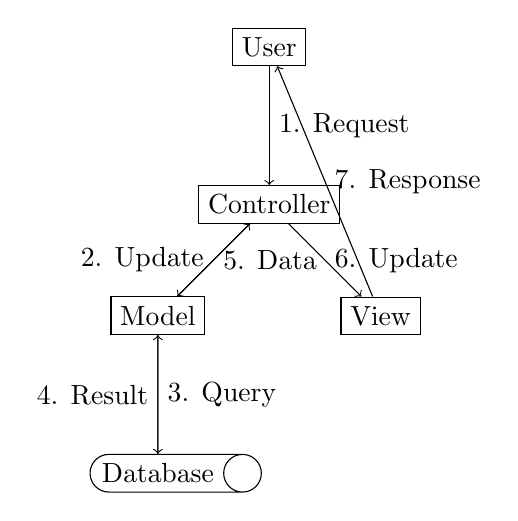
\begin{tikzpicture}[node distance=2cm]
\node (user) [draw, rectangle] {User};
\node (controller) [draw, rectangle, below of=user] {Controller};
\node (model) [draw, rectangle, below left of=controller] {Model};
\node (view) [draw, rectangle, below right of=controller] {View};
\node (database) [draw, cylinder, below of=model] {Database};

\draw[->] (user) -- (controller) node[midway, right] {1. Request};
\draw[->] (controller) -- (model) node[midway, left] {2. Update};
\draw[->] (model) -- (database) node[midway, right] {3. Query};
\draw[->] (database) -- (model) node[midway, left] {4. Result};
\draw[->] (model) -- (controller) node[midway, right] {5. Data};
\draw[->] (controller) -- (view) node[midway, right] {6. Update};
\draw[->] (view) -- (user) node[midway, right] {7. Response};
\end{tikzpicture}

\subsection{Additional Layers}

In addition to the MVC components, the template includes additional layers to improve separation of concerns and maintainability:

\begin{itemize}
    \item \textbf{Repository Layer}: Handles data access operations, abstracting the database interactions from the service layer.
    \item \textbf{Service Layer}: Contains business logic and orchestrates the flow of data between the controllers and repositories.
    \item \textbf{Utility Layer}: Provides helper functions and utilities used throughout the application.
\end{itemize}

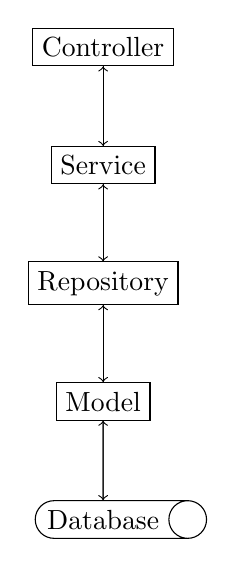
\begin{tikzpicture}[node distance=1.5cm]
\node (controller) [draw, rectangle] {Controller};
\node (service) [draw, rectangle, below of=controller] {Service};
\node (repository) [draw, rectangle, below of=service] {Repository};
\node (model) [draw, rectangle, below of=repository] {Model};
\node (database) [draw, cylinder, below of=model] {Database};

\draw[->] (controller) -- (service);
\draw[->] (service) -- (repository);
\draw[->] (repository) -- (model);
\draw[->] (model) -- (database);
\draw[<-] (model) -- (database);
\draw[<-] (repository) -- (model);
\draw[<-] (service) -- (repository);
\draw[<-] (controller) -- (service);
\end{tikzpicture}

\section{Implementation Details}

\subsection{Application Factory Pattern}

The template uses the application factory pattern to create the Flask application. This pattern allows for better testing and flexibility in creating different instances of the application with different configurations.

\begin{lstlisting}[language=python, caption=Application Factory in app/\_\_init\_\_.py]
def create_app(config_name='default'):
    """Application factory function"""
    app = Flask(__name__)
    
    # Load configuration
    app.config.from_object(config[config_name])
    
    # Initialize extensions
    db.init_app(app)
    migrate.init_app(app, db)
    jwt.init_app(app)
    sess.init_app(app)
    cache.init_app(app)
    limiter.init_app(app)
    csrf.init_app(app)
    
    # Register blueprints
    from app.controllers.auth_controller import auth_bp
    from app.controllers.user_controller import user_bp
    from app.controllers.admin_controller import admin_bp
    from app.controllers.activity_controller import activity_bp
    
    app.register_blueprint(auth_bp, url_prefix='/auth')
    app.register_blueprint(user_bp, url_prefix='/user')
    app.register_blueprint(admin_bp, url_prefix='/admin')
    app.register_blueprint(activity_bp, url_prefix='/activity')
    
    # Configure logging
    if not app.debug and not app.testing:
        if not os.path.exists('logs'):
            os.mkdir('logs')
        file_handler = RotatingFileHandler('logs/flask_app.log', maxBytes=10240, backupCount=10)
        file_handler.setFormatter(logging.Formatter(
            '%(asctime)s %(levelname)s: %(message)s [in %(pathname)s:%(lineno)d]'
        ))
        file_handler.setLevel(logging.INFO)
        app.logger.addHandler(file_handler)
        app.logger.setLevel(logging.INFO)
        app.logger.info('Flask application startup')
    
    # Register error handlers
    @app.errorhandler(404)
    def not_found_error(error):
        return {'error': 'Not found'}, 404
    
    @app.errorhandler(500)
    def internal_error(error):
        db.session.rollback()
        return {'error': 'Internal server error'}, 500
    
    return app
\end{lstlisting}

\subsection{Blueprints}

The template uses Flask blueprints to organize the application into modular components. Each blueprint represents a feature or a set of related features.

\begin{lstlisting}[language=python, caption=Auth Blueprint in app/controllers/auth\_controller.py]
from flask import Blueprint, request, jsonify
from app.services.auth_service import AuthService
from app.utils.decorators import validate_json
from flask_jwt_extended import jwt_required, get_jwt_identity

auth_bp = Blueprint('auth', __name__)

@auth_bp.route('/register', methods=['POST'])
@validate_json('username', 'email', 'password')
def register():
    """Register a new user"""
    data = request.get_json()
    result, status_code = AuthService.register(data)
    return jsonify(result), status_code

@auth_bp.route('/login', methods=['POST'])
@validate_json('username', 'password')
def login():
    """Login a user"""
    data = request.get_json()
    result, status_code = AuthService.login(data)
    return jsonify(result), status_code

@auth_bp.route('/logout', methods=['POST'])
@jwt_required()
def logout():
    """Logout a user"""
    user_id = get_jwt_identity()
    result, status_code = AuthService.logout(user_id)
    return jsonify(result), status_code

@auth_bp.route('/refresh', methods=['POST'])
@validate_json('refresh_token')
def refresh():
    """Refresh access token"""
    data = request.get_json()
    refresh_token = data.get('refresh_token')
    result, status_code = AuthService.refresh_token(refresh_token)
    return jsonify(result), status_code
\end{lstlisting}

\subsection{Models}

The template uses SQLAlchemy ORM to define models. Each model represents a database table and includes relationships to other models.

\begin{lstlisting}[language=python, caption=User Model in app/models/user.py]
from app import db
from datetime import datetime
from werkzeug.security import generate_password_hash, check_password_hash

class User(db.Model):
    """User model for storing user related details"""
    __tablename__ = 'users'

    id = db.Column(db.Integer, primary_key=True)
    username = db.Column(db.String(64), unique=True, nullable=False, index=True)
    email = db.Column(db.String(120), unique=True, nullable=False, index=True)
    password_hash = db.Column(db.String(128), nullable=False)
    role = db.Column(db.String(20), default='user')  # 'user', 'admin'
    is_active = db.Column(db.Boolean, default=True)
    created_at = db.Column(db.DateTime, default=datetime.utcnow)
    updated_at = db.Column(db.DateTime, default=datetime.utcnow, onupdate=datetime.utcnow)
    last_login = db.Column(db.DateTime, nullable=True)
    
    # Relationships
    activities = db.relationship('Activity', backref='user', lazy='dynamic')
    
    @property
    def password(self):
        """Prevent password from being accessed"""
        raise AttributeError('password is not a readable attribute')
    
    @password.setter
    def password(self, password):
        """Set password to a hashed password"""
        self.password_hash = generate_password_hash(password)
    
    def verify_password(self, password):
        """Check if password matches"""
        return check_password_hash(self.password_hash, password)
    
    def is_admin(self):
        """Check if user is admin"""
        return self.role == 'admin'
    
    def __repr__(self):
        return f'<User {self.username}>'
\end{lstlisting}

\subsection{Repositories}

The repository layer abstracts the data access operations from the service layer. Each repository is responsible for performing CRUD operations on a specific model.

\begin{lstlisting}[language=python, caption=User Repository in app/repositories/user\_repository.py]
from app import db
from app.models.user import User
from sqlalchemy.exc import SQLAlchemyError
from typing import List, Optional, Dict, Any

class UserRepository:
    """Repository for User model operations"""
    
    @staticmethod
    def create(user_data: Dict[str, Any]) -> Optional[User]:
        """Create a new user"""
        try:
            user = User(
                username=user_data.get('username'),
                email=user_data.get('email'),
                role=user_data.get('role', 'user')
            )
            user.password = user_data.get('password')
            
            db.session.add(user)
            db.session.commit()
            return user
        except SQLAlchemyError as e:
            db.session.rollback()
            raise e
    
    @staticmethod
    def get_by_id(user_id: int) -> Optional[User]:
        """Get user by ID"""
        return User.query.get(user_id)
    
    @staticmethod
    def get_by_username(username: str) -> Optional[User]:
        """Get user by username"""
        return User.query.filter_by(username=username).first()
    
    @staticmethod
    def get_by_email(email: str) -> Optional[User]:
        """Get user by email"""
        return User.query.filter_by(email=email).first()
    
    @staticmethod
    def get_all(page: int = 1, per_page: int = 20) -> List[User]:
        """Get all users with pagination"""
        return User.query.paginate(page=page, per_page=per_page, error_out=False).items
    
    @staticmethod
    def update(user: User, user_data: Dict[str, Any]) -> Optional[User]:
        """Update user data"""
        try:
            for key, value in user_data.items():
                if key == 'password':
                    user.password = value
                elif hasattr(user, key):
                    setattr(user, key, value)
            
            db.session.commit()
            return user
        except SQLAlchemyError as e:
            db.session.rollback()
            raise e
    
    @staticmethod
    def delete(user: User) -> bool:
        """Delete a user"""
        try:
            db.session.delete(user)
            db.session.commit()
            return True
        except SQLAlchemyError as e:
            db.session.rollback()
            raise e
\end{lstlisting}

\subsection{Services}

The service layer contains business logic and orchestrates the flow of data between the controllers and repositories. Each service is responsible for a specific domain of the application.

\begin{lstlisting}[language=python, caption=Auth Service in app/services/auth\_service.py]
from app.repositories.user_repository import UserRepository
from app.services.token_service import TokenService
from app.services.activity_service import ActivityService
from app.utils.validators import validate_email, validate_password
from typing import Dict, Any, Optional, Tuple
from flask import request

class AuthService:
    """Service for authentication operations"""
    
    @staticmethod
    def register(user_data: Dict[str, Any]) -> Tuple[Dict[str, Any], int]:
        """Register a new user"""
        # Validate input
        if not validate_email(user_data.get('email', '')):
            return {'error': 'Invalid email format'}, 400
        
        if not validate_password(user_data.get('password', '')):
            return {'error': 'Password must be at least 8 characters and contain letters and numbers'}, 400
        
        # Check if user already exists
        if UserRepository.get_by_email(user_data.get('email')):
            return {'error': 'Email already registered'}, 409
        
        if UserRepository.get_by_username(user_data.get('username')):
            return {'error': 'Username already taken'}, 409
        
        # Create user
        try:
            user = UserRepository.create(user_data)
            
            # Log activity
            ActivityService.log_activity(
                user_id=user.id,
                action='user_registered',
                details='User registered successfully',
                request=request
            )
            
            return {'message': 'User registered successfully'}, 201
        except Exception as e:
            return {'error': str(e)}, 500
    
    @staticmethod
    def login(credentials: Dict[str, Any]) -> Tuple[Dict[str, Any], int]:
        """Login a user"""
        username = credentials.get('username')
        password = credentials.get('password')
        
        # Find user by username or email
        user = UserRepository.get_by_username(username)
        if not user:
            user = UserRepository.get_by_email(username)
        
        # Verify user and password
        if not user or not user.verify_password(password):
            return {'error': 'Invalid credentials'}, 401
        
        if not user.is_active:
            return {'error': 'Account is disabled'}, 403
        
        # Update last login
        UserRepository.update_last_login(user)
        
        # Generate tokens
        access_token = TokenService.generate_access_token(user.id, user.role)
        refresh_token = TokenService.generate_refresh_token(user.id)
        
        # Log activity
        ActivityService.log_activity(
            user_id=user.id,
            action='user_login',
            details='User logged in successfully',
            request=request
        )
        
        return {
            'access_token': access_token,
            'refresh_token': refresh_token,
            'user': {
                'id': user.id,
                'username': user.username,
                'email': user.email,
                'role': user.role
            }
        }, 200
\end{lstlisting}

\subsection{Utilities}

The utility layer provides helper functions and utilities used throughout the application. This includes decorators, validators, and security helpers.

\begin{lstlisting}[language=python, caption=Decorators in app/utils/decorators.py]
from functools import wraps
from flask import request, jsonify
from flask_jwt_extended import verify_jwt_in_request, get_jwt
from app.services.authorization_service import AuthorizationService

def admin_required(fn):
    """Decorator to require admin role"""
    @wraps(fn)
    def wrapper(*args, **kwargs):
        verify_jwt_in_request()
        claims = get_jwt()
        if claims.get('role') != 'admin':
            return jsonify(error='Admin access required'), 403
        return fn(*args, **kwargs)
    return wrapper

def permission_required(permission):
    """Decorator to require specific permission"""
    def decorator(fn):
        @wraps(fn)
        def wrapper(*args, **kwargs):
            verify_jwt_in_request()
            claims = get_jwt()
            user_id = claims.get('sub')
            
            if not AuthorizationService.has_permission(user_id, permission):
                return jsonify(error='Permission denied'), 403
            return fn(*args, **kwargs)
        return wrapper
    return decorator

def validate_json(*required_fields):
    """Decorator to validate JSON request data"""
    def decorator(fn):
        @wraps(fn)
        def wrapper(*args, **kwargs):
            if not request.is_json:
                return jsonify(error='Missing JSON in request'), 400
            
            data = request.get_json()
            missing_fields = [field for field in required_fields if field not in data]
            
            if missing_fields:
                return jsonify(error=f'Missing required fields: {", ".join(missing_fields)}'), 400
            
            return fn(*args, **kwargs)
        return wrapper
    return decorator
\end{lstlisting}

\section{Authentication and Authorization}

\subsection{JWT Authentication}

The template uses JWT (JSON Web Tokens) for authentication. When a user logs in, they receive an access token and a refresh token. The access token is used to authenticate API requests, while the refresh token is used to obtain a new access token when the current one expires.

\begin{lstlisting}[language=python, caption=Token Service in app/services/token\_service.py]
from flask_jwt_extended import create_access_token, create_refresh_token, decode_token
from typing import Dict, Any, Optional
from datetime import datetime, timezone
import jwt
from flask import current_app

class TokenService:
    """Service for JWT token operations"""
    
    @staticmethod
    def generate_access_token(user_id: int, role: str) -> str:
        """Generate JWT access token"""
        return create_access_token(
            identity=user_id,
            additional_claims={'role': role}
        )
    
    @staticmethod
    def generate_refresh_token(user_id: int) -> str:
        """Generate JWT refresh token"""
        return create_refresh_token(identity=user_id)
    
    @staticmethod
    def verify_access_token(token: str) -> Optional[Dict[str, Any]]:
        """Verify JWT access token"""
        try:
            return decode_token(token)
        except Exception:
            return None
    
    @staticmethod
    def verify_refresh_token(token: str) -> Optional[Dict[str, Any]]:
        """Verify JWT refresh token"""
        try:
            return decode_token(token)
        except Exception:
            return None
\end{lstlisting}

\subsection{Role-Based Access Control}

The template implements role-based access control (RBAC) to restrict access to certain resources based on the user's role. The AuthorizationService defines permissions for each role and provides methods to check if a user has a specific permission.

\begin{lstlisting}[language=python, caption=Authorization Service in app/services/authorization\_service.py]
from app.repositories.user_repository import UserRepository
from typing import Dict, Any, List, Optional

class AuthorizationService:
    """Service for authorization operations"""
    
    # Define permission constants
    PERMISSIONS = {
        'user': [
            'profile:read',
            'profile:update',
            'activity:read_own'
        ],
        'admin': [
            'profile:read',
            'profile:update',
            'profile:read_any',
            'profile:update_any',
            'profile:delete_any',
            'activity:read_own',
            'activity:read_any',
            'user:create',
            'user:read',
            'user:update',
            'user:delete'
        ]
    }
    
    @staticmethod
    def get_permissions(role: str) -> List[str]:
        """Get permissions for a role"""
        return AuthorizationService.PERMISSIONS.get(role, [])
    
    @staticmethod
    def has_permission(user_id: int, permission: str) -> bool:
        """Check if user has a specific permission"""
        user = UserRepository.get_by_id(user_id)
        if not user:
            return False
        
        user_permissions = AuthorizationService.get_permissions(user.role)
        return permission in user_permissions
    
    @staticmethod
    def can_access_resource(user_id: int, resource_owner_id: int, permission: str) -> bool:
        """Check if user can access a specific resource"""
        # If user is the resource owner, check for own permission
        if user_id == resource_owner_id:
            return True
        
        # Otherwise, check for any permission
        return AuthorizationService.has_permission(user_id, permission)
\end{lstlisting}

\section{Activity Tracking}

The template includes activity tracking to log user actions. This is useful for auditing and debugging purposes. The ActivityService provides methods to log activities and retrieve activity logs.

\begin{lstlisting}[language=python, caption=Activity Service in app/services/activity\_service.py]
from app.repositories.activity_repository import ActivityRepository
from flask import Request
from typing import Dict, Any, List, Optional

class ActivityService:
    """Service for activity tracking operations"""
    
    @staticmethod
    def log_activity(user_id: int, action: str, details: Optional[str] = None, 
                    request: Optional[Request] = None) -> Dict[str, Any]:
        """Log a user activity"""
        activity_data = {
            'user_id': user_id,
            'action': action,
            'details': details
        }
        
        # Add request information if available
        if request:
            activity_data['ip_address'] = request.remote_addr
            activity_data['user_agent'] = request.user_agent.string
        
        try:
            activity = ActivityRepository.create(activity_data)
            return {
                'id': activity.id,
                'user_id': activity.user_id,
                'action': activity.action,
                'timestamp': activity.timestamp.isoformat()
            }
        except Exception as e:
            # Log the error but don't fail the main operation
            print(f"Error logging activity: {str(e)}")
            return {}
\end{lstlisting}

\section{Security Features}

\subsection{Password Hashing}

The template uses Werkzeug's password hashing functions to securely store passwords. Passwords are never stored in plain text.

\begin{lstlisting}[language=python, caption=Password Hashing in app/models/user.py]
@property
def password(self):
    """Prevent password from being accessed"""
    raise AttributeError('password is not a readable attribute')

@password.setter
def password(self, password):
    """Set password to a hashed password"""
    self.password_hash = generate_password_hash(password)

def verify_password(self, password):
    """Check if password matches"""
    return check_password_hash(self.password_hash, password)
\end{lstlisting}

\subsection{CSRF Protection}

The template includes CSRF protection using Flask-WTF. This helps prevent cross-site request forgery attacks.

\begin{lstlisting}[language=python, caption=CSRF Protection in app/\_\_init\_\_.py]
from flask_wtf.csrf import CSRFProtect

csrf = CSRFProtect()

def create_app(config_name='default'):
    # ...
    csrf.init_app(app)
    # ...
\end{lstlisting}

\subsection{Rate Limiting}

The template includes rate limiting using Flask-Limiter. This helps prevent brute-force attacks and abuse.

\begin{lstlisting}[language=python, caption=Rate Limiting in app/\_\_init\_\_.py]
from flask_limiter import Limiter
from flask_limiter.util import get_remote_address

limiter = Limiter(key_func=get_remote_address)

def create_app(config_name='default'):
    # ...
    limiter.init_app(app)
    # ...
\end{lstlisting}

\section{Caching}

The template includes caching using Flask-Caching. This helps improve performance by caching frequently accessed data.

\begin{lstlisting}[language=python, caption=Cache Service in app/services/cache\_service.py]
from app import cache
from typing import Any, Optional
from datetime import timedelta

class CacheService:
    """Service for cache operations"""
    
    @staticmethod
    def set(key: str, value: Any, timeout: Optional[int] = None) -> bool:
        """Set a cache value"""
        return cache.set(key, value, timeout=timeout)
    
    @staticmethod
    def get(key: str, default: Any = None) -> Any:
        """Get a cache value"""
        value = cache.get(key)
        return value if value is not None else default
    
    @staticmethod
    def delete(key: str) -> bool:
        """Delete a cache value"""
        return cache.delete(key)
    
    @staticmethod
    def clear() -> bool:
        """Clear all cache"""
        return cache.clear()
    
    @staticmethod
    def has(key: str) -> bool:
        """Check if cache has a key"""
        return cache.has(key)
    
    @staticmethod
    def memoize(timeout: Optional[int] = None):
        """Decorator to memoize a function"""
        return cache.memoize(timeout=timeout)
    
    @staticmethod
    def cached(timeout: Optional[int] = None, key_prefix: str = 'view'):
        """Decorator to cache a view function"""
        return cache.cached(timeout=timeout, key_prefix=key_prefix)
\end{lstlisting}

\section{Session Management}

The template includes session management using Flask-Session. This allows for server-side session storage, which is more secure than client-side cookies.

\begin{lstlisting}[language=python, caption=Session Service in app/services/session\_service.py]
from flask import session
from typing import Any, Optional
from datetime import datetime, timedelta

class SessionService:
    """Service for session management"""
    
    @staticmethod
    def set(key: str, value: Any, expiry: Optional[timedelta] = None) -> None:
        """Set a session value"""
        session[key] = value
        
        # Set expiry if provided
        if expiry:
            session[f"{key}_exp"] = (datetime.utcnow() + expiry).timestamp()
    
    @staticmethod
    def get(key: str, default: Any = None) -> Any:
        """Get a session value"""
        # Check expiry if it exists
        expiry_key = f"{key}_exp"
        if expiry_key in session:
            expiry = session[expiry_key]
            if datetime.utcnow().timestamp() > expiry:
                # Expired, remove and return default
                SessionService.remove(key)
                return default
        
        return session.get(key, default)
    
    @staticmethod
    def remove(key: str) -> None:
        """Remove a session value"""
        if key in session:
            session.pop(key)
        
        # Remove expiry if it exists
        expiry_key = f"{key}_exp"
        if expiry_key in session:
            session.pop(expiry_key)
    
    @staticmethod
    def clear() -> None:
        """Clear all session data"""
        session.clear()
    
    @staticmethod
    def has(key: str) -> bool:
        """Check if session has a key"""
        return key in session
\end{lstlisting}

\section{Conclusion}

This technical report has provided a comprehensive overview of the Flask MVC Template with MySQL. The template follows the MVC architectural pattern and includes additional layers to improve separation of concerns and maintainability. It includes features such as authentication, authorization, activity tracking, caching, session management, and security features. The template provides a solid foundation for building web applications with Flask.

\end{document}

